\documentclass{article}

\usepackage{graphicx}
\usepackage{hyperref}
\usepackage{listings}
\usepackage{color}
\usepackage{verbatim}
\usepackage{amsmath}


\linespread{1.5}
\begin{document}

\section{Background}
\subsection{Graph Laplacian Problem}
Information about a weighted, undirected graph $G$ with vertex list $V$ and edge list $E$ can be stored in a matrix. This is called the adjacency matrix which is defined as:\\
\begin{center} 
$A(u,v) = 1$ if $(u,v) \in E$ and $0$ otherwise.\\
\end{center}
The diagonal matrix, $D$ is a matrix of the degree sequence along the diagonal:\\
\begin{center}
$D(u,u) = d_u$
\end{center}
The laplacian matrix is $L = D-A$. This is done because it is similar to the finite difference discretization of the laplacian on a grid.\\
\begin{figure}
\begin{center}
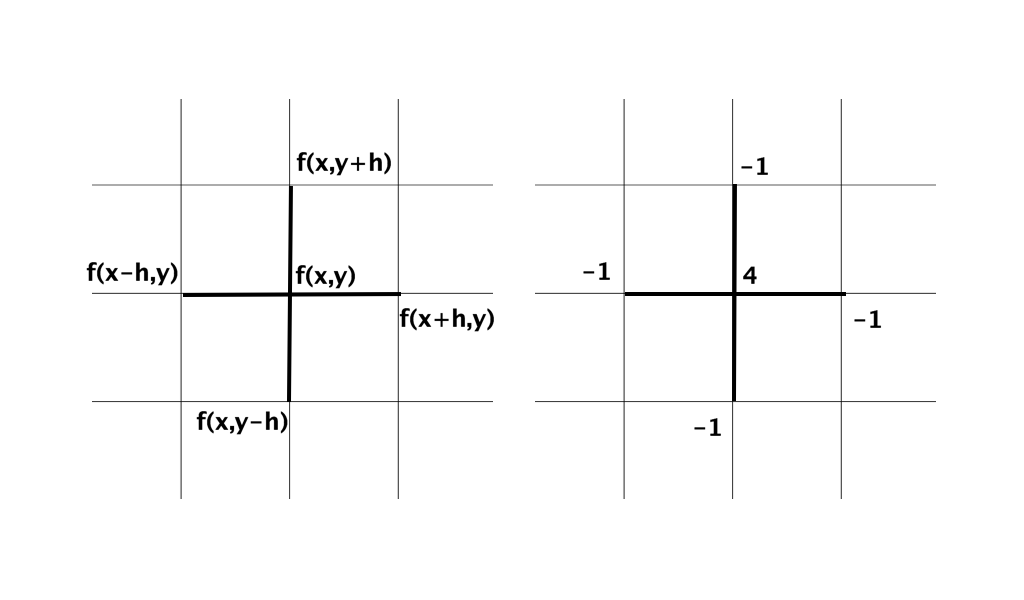
\includegraphics[width=\linewidth]{laplace.png}
  \caption{Finite difference discretization on a grid}
  \end{center}
  \end{figure}\\
 
The 3D finite difference discretization is similar because each edge contributes two terms: one to the adjacency matrix and one to the diagonal matrix. This is how we build multidimensional graph Laplacians.
To see how information flows through paths in a network, the graph laplacian matrix can be used as an operator on an input vector. To find a weighted average of paths in a network one can repeatedly apply the Laplacian operator on an input. This results in a Neumann Series with inverse defined if the series converges in the operator norm \cite{Neumann:1877,Kantorovich:1982}:\\
\begin{center}
$b + Lb + L^{2}b + L^{3}b + L^{4}b + ... = \sum_{i = 0}^{\infty} L^{i}b = (I-L)^{-1}b$\\
\end{center}
Thus in problems related to graph regression, spectral graph theory, maximum and minimum cost flow, resistor networks, and partial differential equations it is common to use the inverse operator of the graph laplacian. \cite{Spielman:2010}

\subsection{Current Solution Approaches}
Solution algorithms for linear systems can be divided into direct methods and iterative methods. Standard direct methods such as $LU$ or Cholesky factorization are accurate and suitable for graphs with small numbers of edges/vertices, however become very costly in terms of memory and time as the size and edge density of the graph increases. Fast matrix inversion can be applied with order $O(N^{2.376})$ \cite{Spielman:2010}. Alternatively one can use nested dissection, however computational memory requirements blow up as size increases; 2D meshes require $O(N log N)$ memory, 3D requires $O(N^{\frac{4}{3}})$ memory and the requirements are greater for highly connected power-law graphs\cite{Khaira:1992}. In contrast to direct solvers, iterative methods compute better and better approximate solutions to the linear system. A standard iterative method is the Conjugate Gradient method \cite{Hestenes:1952}. To speed up these iterative methods, it is possible to introduce a preconditioner that creates an equivalent linear system that is much easier to solve than the original \cite{Saad:2003}. Yet none of these basic solvers take into account attributes of the graph Laplacian that can drastically improve method performance.

\subsubsection{Spielman-Teng, Koutis et. al.}
As an analogy with preconditioning, we want to find an approximation to a graph $G$ with similar spectrum for easier computing. Spielman and Teng introduce the idea of a spectral sparsifier. The Laplacian for this approximation is similar to the Laplacian for the original graph because of similar spectrum, thus resulting in a good preconditioner for the original linear system. Multiple cycles of sparsification and factorization combine to solve the original problem. They have a multilevel version of this. Spielman and Teng (S-T) were thus able to solve symmetric diagonally dominant systems in nearly linear time \cite{Spielman:2008}.  This line of work combined with Vaidya's \cite{Vaidya:1991} work on subgraph preconditioners (capacitance matrix methods) resulted in Koutis and Miller's work solving linear systems based on planar Laplacians \cite{Koutis:2007}. Koutis, et. al. were able to extend the results to general symmetric diagonally dominant systems \cite{Koutis:2010}.

\subsection{Multigrid Approaches}
Algebraic Multigrid creates a coarse basis through agglomeration and then uses a Galerkin operator in multiple graph coarsening cycles to solve a linear system. It is mostly used to solve discretized partial differential equations, but has also become more popular in solving graph Laplacian systems. AMG can have optimal time complexity and demonstrates good parallel scaling, thus it is useful for solving incredibly large problems \cite{Livne:2012}. Straightforward AMG on these graphs is not optimal because it cannot coarsen the graphs fast enough. So three multigrid approaches to the graph Laplacian problem with heuristics for coarsening are combinatorial multigrid (CMG) from Koutis et. al. \cite{Koutis:2011}, Cascadic multigrid from Urschel et. al. \cite{Urschel:2014}, and Lean Algebraic Multigrid (LAMG) from Livne and Brandt \cite{Livne:2012}. All three propose coarsening over the entire graph with ideas for how to aggregate edge information. But an important question to ask is: how do you coarsen a graph with edges of varying degrees? How do you know which edges or vertices can be aggregated and still preserve information?


\subsubsection{Combinatorial Multigrid (CMG)}
Koutis, Miller, and Tolliver propose a combinatorial multigrid solver to solve computer vision problems. This method creates a two-level iterative approach combining the previously mentioned subgraph preconditioning work of Vaidya with algebraic multigrid. For a set of increasingly larger three-dimensional images, CMG required less iterations to converge than a standard multigrid solver in Matlab \cite{Koutis:2011}.

\subsubsection{Lean Algebraic Multigrid (LAMG)}
Livne and Brandt ran a 'lean' multigrid algorithm on graph Laplacian systems for almost 4000 real world graphs of varying size and in vastly different fields from the natural sciences to social networks. Their method has three key parts: first, vertices with low degree are eliminated before the graph is coarsened. Second: they aggregate vertices for the coarsening by a proximity heuristic. And third: they apply an energy correction to the Galerkin operator and take linear combinations of solutions to
accelerate the iteration. They test their algorithm against CMG, and find that it requires slightly more work, however is more robust overall \cite{Livne:2012}. One potential downside of LAMG is
the heuristics used in the vertex aggregation step. How can vertices be evenly aggregated over graphs with uneven degree distribution?


\subsubsection{Cascadic Multigrid}
A final alternative form of multigrid was proposed by Urshel et. al. to solve a related problem to the graph Laplacian linear system; they wanted to calculate the Fiedler vector (eigenvector corresponding to the second smallest eigenvalue) of a graph Laplacian. This cascadic multigrid utilizes heavy edge maching to quickly coarsen a graph \cite{Urschel:2014}. It remains to be seen whether this approach will be successful for solving an entire Laplacian linear system accurately.

\subsection{Graph Partitioning and Multigrid}
I have studied the methods of graph partitioning and sparsification for solving linear systems, and using multigrid to solve the graph laplacian linear system specifically. I combine these two approaches using Chung and Lu's work \cite{Chung:2004} and optimal multigrid to solve similar linear systems.
%\bibliographystyle{siam}
%\bibliography{mastersbib}


\end{document}